\documentclass{beamer}
\usepackage{amssymb}
\usepackage{graphicx}
\usetheme{Berlin}


\title[Emisi\'on de la fotosfera]{\textbf{Emisi\'on de la fotosfera}}
\author{Antonio Galv\'an}
\date{5 Mayo 2014}
\institute{Instituto de Astronom\'ia\\ Facultad
 de Ciencias\\ U.N.A.M.}

\begin{document}
\begin{frame}
\titlepage
\end{frame}

\begin{frame}
\frametitle{\'Indice}
\tableofcontents[pausesections]
\end{frame}

\section{Introducci\'on}

\begin{frame}
\frametitle{Introducci\'on:} 
Se cree a lo largo de muchas observaciones que los GRB's surgen 
de la disipaci\'on de energ\'ia cin\'etica de un flujo relativista,
 original de un objeto central compacto.\\
Esta energ\'ia disipada es convertida en electrones energ\'eticos que
producen fotones altamente energ\'eticos por medio de radiaci\'on Sincrotron y 
Compton Inverso.
\end{frame}

\subsection{Y la fotosfera ?`qu\'e rol tiene?}
\begin{frame}
\frametitle{?`Y la fotosfera ¿qu\'e rol tiene?}
	\begin{columns}
	
		\begin{column}{5cm}
		En un modelo c\'omo lo es el termonuclear en el que propone que el material acretado
		de un sistema binario o de una estrella de neutrones peque\~na con un entorno altamente
		denso.
		\end{column}
		
		\begin{column}{5cm}
		En el modelo de la estrella de neutrones formada por una capa de hidr\'ogeno (H) en la capa
		m\'as externa, seguida de una capa de helio (He) y metales por debajo de \'esta con una densidad
		de $10^{7}g cm^{-2}$ y $T\backsim 10^{7}K $ los electrones se degeneran.\\
		De esta manera se genera una combusti\'on nuclear.
		\end{column}	
	\end{columns}
\end{frame}

\begin{frame}
	\begin{columns}
	
		\begin{column}{5cm}
			\begin{figure}
				\centering
				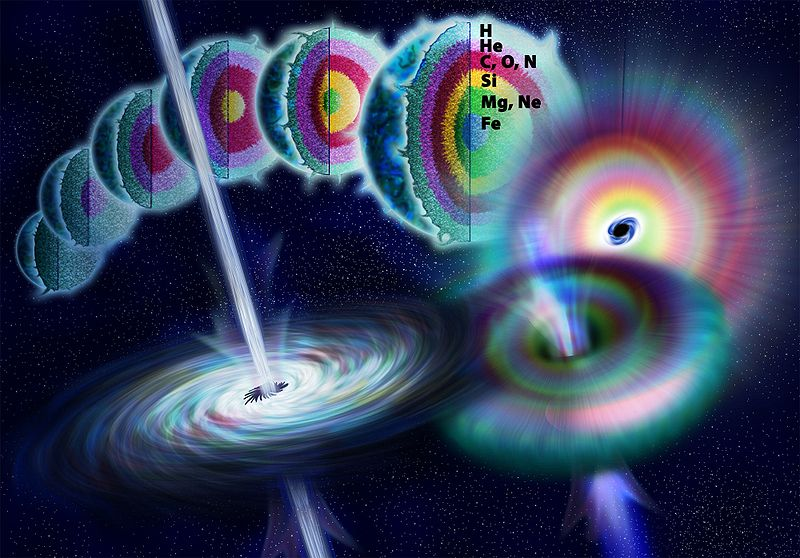
\includegraphics[scale=0.75]{neutronStar.jpg}
				\caption{Distintos procesos de la estrella de neutrones.}
			
			\end{figure}
		\end{column}
		
		\begin{column}{5cm}
		De tal forma de que el hidr\'ogeno se  por CNO no limitado y por medio de electrones 
		capturados por protones. Cu\'ando la temperatura alcanza $\backsim 10^{8}K $ la capa de (He)
		explota generando la cantidad necesaria para originar un GRB.
		\end{column}	
	\end{columns}
\end{frame}



\end{document}
